\documentclass[11pt]{article}

\usepackage[english]{babel}         % American English
\usepackage[T1]{fontenc}            % Required for hyphenation
\usepackage[utf8]{inputenc}         % UTF-8 encoding

\usepackage{amssymb,amsmath,amsthm} % AMS
\allowdisplaybreaks                 % Math displays can break
\usepackage{url}                    % Typesetting URLs
\usepackage{hyphenat}               % Hyphenation with \hyp
\usepackage[scaled=0.8]{beramono}   % Nice bold/italic teletype font
\usepackage{float}                  % Tuning placement of figures
\usepackage{graphicx}               % Inclusion of graphics
\usepackage{caption,subfig}         % Subfigures
\usepackage{xspace}                 % Proper spacing after macros
\usepackage{alltt,calc}             % Verbatim with macros
\captionsetup[subfloat]{justification=raggedleft}
\usepackage[justification=raggedleft]{caption}
\usepackage{wrapfig}                % Wrapping text around figures
\usepackage[colorlinks=true,citecolor=black,linkcolor=black,urlcolor=blue]{hyperref}

\bibliographystyle{plain}  % TEMPORARY
%\usepackage{etoolbox}
%\apptocmd{\thebibliography}{\raggedright}{}{} % No Underfull \hbox

% New commands
%
\newcommand{\nb}[1]{\marginpar{{\color{red}\small #1}}}
\newcommand{\XML}{\textsf{XML}\xspace}
\newcommand\fig{\textsc{Figure}}
\newcommand\Fig{\textsc{Figure}}
%\renewcommand{\cdot}{\,}
\newcommand{\A}[2]{H_{#1}^{<#2}}
\newcommand{\B}[2]{H_{#1}^{\geqslant #2}}
\newcommand\Expected[1]{\mathbb{E}[{#1}]}

\title{A Purely Combinatorial Derivation of the Average Height of
  Catalan Trees}
\author{Nachum Dershowitz \and Christian Rinderknecht}
\date{}

\begin{document}

\maketitle

The present note is the online supplement
to~\cite{DershowitzRinderknecht:2015}, which simplified the analytical
derivation of the average height of Catalan trees. Here, we propose an
alternate approach to obtain the same result, but by purely
combinatorial means.

We are going to proceed in two steps: first, we will bound the average
height in terms of the average distance of a random node from the
root; second, we will determine the latter, yielding the result only
by combinatorial means.

\section{Average height}

We have already seen the correspondence between lattice paths and
Catalan trees, in which a rise reaching the $l$th diagonal corresponds
to a node at level~$l$ in the tree, counting levels from root
level~$0$.  A simple bijection between paths will show that for every
node on level~$l$ of a tree of height~$h$ and size~$n$, there is a
corresponding node on either level $h-l$ or $h-l-1$ in another tree of
the same height and size.

Consider the Dyck path in~\Fig~\ref{fig:h},
\begin{figure}
\centering
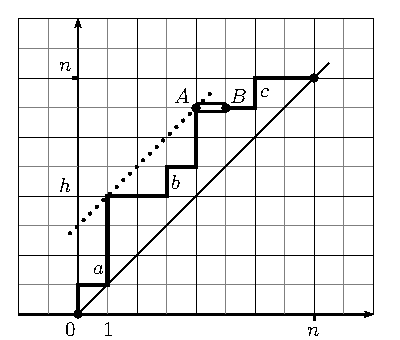
\includegraphics{h}
\caption{A Dyck path of length~\(2n\) and height~\(h-1\)\label{fig:h}}
\end{figure}
in bijection with a tree with~\(n=8\) edges and height~\(h=4\). Let us
find the last (rightmost) point on the path where it reaches its full
height (the dotted line of equation \(y = x + h - 1\)), which we call
the \emph{apex} of the path (marked~$A$ in the figure).  The
immediately following fall leads to~$B$ and it is drawn with a double
line. Let us rotate the segment from $(0,0)$ to~$A$, and the segment
from~$B$ to~$(n,n)$ by 180$^\circ$. The invariant fall $(A,B)$ now
connects the rotated segments. This way, what was the apex becomes the
origin and vice\hyp{}versa, making this a height\hyp{}preserving
bijection between paths. See \fig~\ref{fig:h_prime}.
\begin{figure}[!t]
\centering
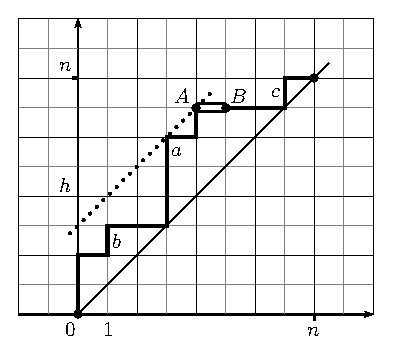
\includegraphics{h_prime}
\caption{Dyck path in bijection with \fig~\ref{fig:h}
\label{fig:h_prime}}
\end{figure}

The point is that every rise to level~$l$ in \fig~\ref{fig:h},
representing a node on level~$l$, ends up reaching level $h-l$ or
$h-l-1$ in \fig~\ref{fig:h_prime}, depending on whether it was to the
left (segment before~$A$) or right (segment after~$B$) of the apex.
In the example in the figure, the rise~$a$ reaches level~$1$, and its
counterpart after the transformation rises to level \(4-1=3\); the
rise~$b$ reached level~$2$ and still does so because \(4-2=2\); the
rise~$c$ also reached level~$2$, but because it was to the right of
the apex, it reaches now level \(4-2-1=1\).  It follows from this
bijection that \emph{the average height of trees with~$n$ nodes is
  within one of twice the average level of a node.}

We now have to determine the average level of a node in order to
conclude. For this, we investigate the average path length of a tree.

\section{Average path length}

The \emph{path length} of a Catalan tree is the sum of the lengths of
the paths from the root. In order to study the average path length, we
will follow Dershowitz and Zaks~\cite{DershowitzZaks:1981} in finding
first the average number of nodes of degree~\(d\) at level~\(l\) in a
Catalan tree with \(n\)~edges, where the \emph{degree of a node} is
the number of its children (the number of nodes immediately below it).

\subsection{Degree-based bijection}

The first step of our method for finding the average path length
consists in finding an alternative bijection between Catalan trees and
Dyck paths. In \fig~\ref{fig:ctree},
\begin{figure}
\centering
\subfloat[Dyck path of length 12.\label{fig:dyck}]{%
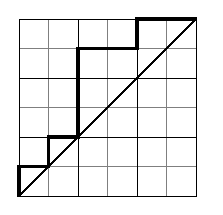
\includegraphics[bb=60 634 167 721]{dyck}
}
\qquad\qquad
\subfloat[Catalan tree with 6 edges.\label{fig:ctree}]{%
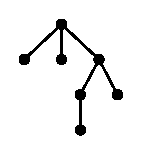
\includegraphics[bb=60 663 138 721,scale=1.5]{ctree}
}
\caption{Bijection between Dyck paths and Catalan trees.\label{fig:bijection}}
\end{figure}
we can see a Catalan tree equivalent to the Dyck path in
\fig~\ref{fig:dyck}, built from the preorder traversal of that
tree. \Fig~\ref{fig:ctree_deg}
\begin{figure}[b]
\centering
\subfloat[Dyck path\label{fig:dyck_deg}]{%
  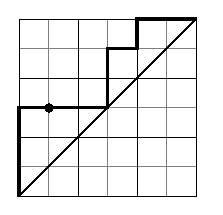
\includegraphics[bb=71 634 158 712]{dyck_deg}}
\qquad
\subfloat[Catalan tree\label{fig:ctree_deg}]{%
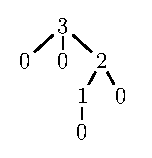
\includegraphics[bb=65 663 127 721]{ctree_deg}
}
\caption{Degree-based bijection}
\end{figure}
shows the same tree, where the contents of the nodes are their
degree. The preorder traversal (of the degrees) is \((3, 0, 0, 2, 1,
0, 0)\). Since the last degree is always~\(0\) (a leaf), we remove it
and settle for \((3, 0, 0, 2, 1, 0)\). Another equivalent Dyck path
may be obtained by mapping the degrees of that list into as many
occurrences of rises (\(\uparrow\)) and one fall (\(\rightarrow\)),
so, for instance, \(3\)~is mapped to \(\uparrow\) \(\uparrow\)
\(\uparrow\) \(\rightarrow\) and \(0\)~to~\(\rightarrow\). In the end,
\((3,0,0,2,1,0)\) is mapped into \(\uparrow\) \(\uparrow\)
\(\uparrow\) \(\rightarrow\) \(\rightarrow\) \(\rightarrow\)
\(\uparrow\) \(\uparrow\) \(\rightarrow\) \(\uparrow\) \(\rightarrow\)
\(\rightarrow\), which corresponds to the Dyck path in
\fig~\ref{fig:dyck_deg}. It is easy to convince ourself that we can
reconstruct the tree from the Dyck path, so we indeed have a
bijection.

The reason for this new bijection is that we need to find the average
number of Catalan trees whose root has a given degree. This number
will help us in finding the average path length, following an idea of
Ruskey~\cite{Ruskey:1983}. From the bijection, it is clear that the
number of trees whose root has degree~\(r=3\) is the number of Dyck
paths made of the segment from \((0,0)\) to \((0,r)\), followed by one
fall (see the dot at \((1,r)\) in \fig~\ref{fig:dyck_deg}), and then
all monotonic paths above the diagonal until the upper right corner
\((n,n)\). Therefore, we need to determine the number of such paths.

\subsection{Path reversal}

We already have seen a bijection called \emph{reflection}, shown in
\fig~\ref{fig:reflection}.
\begin{figure}[b]
\centering
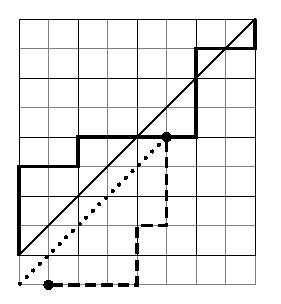
\includegraphics[scale=0.9]{reflection}
\caption{Reflection of a prefix with respect to \(y = x - 1\).
\label{fig:reflection}}
\end{figure}
Let us add to our tool box one more bijection which often proves
useful: \emph{reversal}. It simply consists in reversing the order of
the steps making up a path. Consider for example
\fig~\ref{fig:path_reversal}.
\begin{figure}
\centering
\subfloat[Reversal of
\fig~\ref{fig:reflection} \label{fig:path_reversal}]{
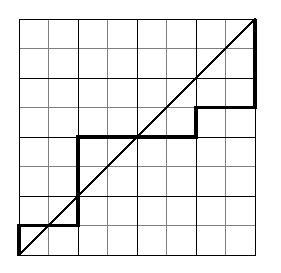
\includegraphics[bb=71 606 188 721]{path_reversal}}
\qquad
\subfloat[Reversal and reflection of \fig~\ref{fig:dyck_deg} after \((1,3)\)\label{fig:path_deg}]{
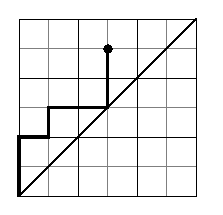
\includegraphics[bb=71 634 162 721]{path_deg}}
\caption{Reversals and reflections}
\end{figure}
Of course, the composition of two bijections being a bijection, the
composition of a reversal and a reflection is bijective, hence the
monotonic paths above the diagonal from \((1,r)\) to \((n,n)\) are in
bijection with the monotonic paths above the diagonal from \((0,0)\)
to \((n-r,n-1)\). For example, \fig~\ref{fig:path_deg} shows the
reversal and reflection of the Dyck path of \fig~\ref{fig:dyck_deg}
after the point \((1,3)\), distinguished by the black disk
(\(\bullet\)).

\subsection{Counting trees by root degree}

\hspace{-4pt} Recalling that Catalan trees with \(n\)~edges are in
bijection with Dyck paths of length~\(2n\), we now know that the
number of Catalan trees with \(n\)~edges and whose root has
degree~\(r\) is the number of monotonic paths above the diagonal from
the point \((0,0)\) to \((n-r,n-1)\). We can find this number using
the same technique we used for the total number~\(C_n\) of Dyck
paths. The principle of inclusion and exclusion says that we should
count the total number of paths with the same extremities and retract the
number of paths that cross the diagonal. The former is
\(\binom{2n-r-1}{n-1}\), which enumerates the ways to interleave
\(n-1\)~rises (\(\uparrow\)) and \(n-r\) falls (\(\rightarrow\)). The
latter number is the same as the number of monotonic paths from
\((1,-1)\) to \((n-r,n-1)\), as shown by reflecting the paths up to
their first crossing, that is, \(\binom{2n-r-1}{n}\); in other words,
that is the number of interleavings of \(n\)~rises with \(n-r-1\)
falls. Finally, imitating the derivation of
\begin{equation}
C_n = \frac{1}{n+1}\binom{2n}{n} \sim \frac{4^n}{n\sqrt{\pi n}},
      \quad\text{as \(n \rightarrow \infty\)}.
\label{eq:Cn}
\end{equation}
(see section \emph{Counting Catalan trees} in the main article), we
find the number \(\mathcal{R}_n(r)\) of trees with \(n\)~edges and
root of degree~\(r\) is
\begin{equation}
\mathcal{R}_n(r) = \binom{2n-r-1}{n-1} - \binom{2n-r-1}{n}.
%                 = \frac{r}{2n-r} \binom{2n-r}{n}.
\label{eq:R_n}
\end{equation}

\subsection{Counting trees by node level and degree}

Let \(\mathcal{N}_n(l,d)\) be the number of Catalan trees with
\(n\)~edges at level~\(l\) and of
degree~\(d\). Ruskey~\cite{Ruskey:1983} found a neat bijection to
relate it to \(\mathcal{R}_n(r)\) by the following equation:
\begin{equation}
\mathcal{N}_n(l,d) = \mathcal{R}_{n+l}(2l+d).
\label{eq:Ruskey}
\end{equation}
\Fig~\ref{fig:level_deg}
\begin{figure}
\centering
\subfloat[\(n\)~edges, (\(\bullet\)) is of degree~\(d\) and at level~\(l\) \label{fig:level_deg}]{%
  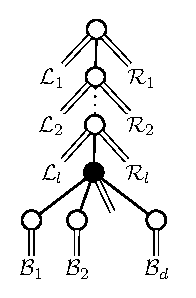
\includegraphics[bb=71 594 150 721]{level_deg}}
\quad
\subfloat[\(n+l\) edges, root of degree~\(2l+d\)\label{fig:lifted_node}]{%
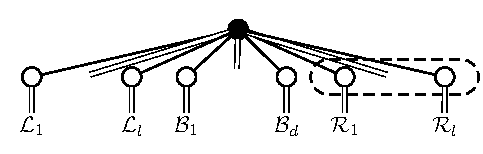
\includegraphics[bb=71 663 295 721]{lifted_node}
}
\caption{Bijection\label{fig:bij_root_level}}
\end{figure}
depicts the general pattern of a Catalan tree with node (\(\bullet\))
of level~\(l\) and degree~\(d\). The double edges denote a set of
edges, so the \(\mathcal{L}_i\), \(\mathcal{R}_i\) and
\(\mathcal{B}_i\) actually represent forests. In
\fig~\ref{fig:lifted_node}, we see a Catalan tree in bijection with the
former, from which it is made by lifting the node of interest
(\(\bullet\)) to become the root, the forests \(\mathcal{L}_i\) with
their respective parents are attached below it, then the
\(\mathcal{B}_i\), and, finally, the \(\mathcal{R}_i\) for which new
parents are needed (inside a dashed frame in the figure). Clearly, the
new root is of degree \(2l+d\) and there are \(n+l\)
edges. Importantly, the transformation can be inverted for any tree
(it is injective and surjective), so it is indeed a
bijection. From~\eqref{eq:R_n} and~\eqref{eq:Ruskey}, we deduce
\begin{equation}
\mathcal{N}_n(l,d) %= \frac{2l+d}{2n-d}\binom{2n-d}{n+l}
= \binom{2n-d-1}{n+l-1} - \binom{2n-d-1}{n+l}.
\label{eq:N_n_l_d}
\end{equation}

\subsection{Average level of a node}

Let \(\Expected{P_n}\) be the \emph{average path length} of a Catalan
tree with \(n\)~edges. We have
\begin{equation}
  \Expected{P_n} := \frac{1}{C_{n}} \,
  \sum_{l=0}^{n}l\sum_{d=0}^{n}\mathcal{N}_n(l,d),
\label{eq:P_n}
\end{equation}
because there are \(C_n\)~trees and the double summation is the sum of
the path lengths of all the trees with~\(n\) edges. If we average
again by the number of nodes, \emph{i.e.,} \(n+1\), we obtain the
average level of a node in a random Catalan tree.  In particular,
equation~\eqref{eq:N_n_l_d} entails that the total number of nodes at
level~\(l\) in all Catalan trees with \(n\)~edges is
\begin{equation}
\sum_{d=0}^{n}\mathcal{N}_n(l,d)
  = \sum_{d=0}^{n}\binom{2n-d-1}{n+l-1}
    - \sum_{d=0}^{n}\binom{2n-d-1}{n+l}.
\label{eq:sum_N_n}
\end{equation}
Let us consider the first sum:
\begin{equation*}
\sum_{d=0}^{n}\binom{2n-d-1}{n+l-1}
  = \sum_{i=n-1}^{2n-1}\binom{i}{n+l-1}
  = \sum_{i=n+l-1}^{2n-1}\binom{i}{n+l-1}.
\end{equation*}
We have the derivation
\begin{align*}
\binom{n+m}{n+1}
  &= \binom{n+m-1}{n} + \binom{n+m-1}{n+1}\notag\\
  &= \binom{n+m-1}{n} + \left[\binom{n+m-2}{n} +
     \binom{n+m-2}{n+1}\right]\notag\\
  &= \binom{n+m-1}{n} + \binom{n+m-2}{n} + \dots +
     \left[\binom{n}{n} + \binom{n}{n+1}\right],\notag\\
\binom{n+m}{n+1}
  &= \sum_{j=0}^{m-1}{\binom{n+j}{n}}.
\end{align*}
This identity is equivalent to \(\sum_{i=j}^{k}\binom{i}{j} =
\binom{k+1}{j+1}\), so \(j=n+l-1\) and \(k=2n-1\) yields
\begin{equation*}
\sum_{d=0}^{n}\binom{2n-d-1}{n+l-1} = \binom{2n}{n+l}.
\end{equation*}
Furthermore, replacing \(l\)~by \(l+1\) gives
\(\sum_{d=0}^{n}\binom{2n-d-1}{n+l} = \binom{2n}{n+l+1}\), so we can
now resume from equation~\eqref{eq:sum_N_n} and find the total number
of nodes at level~\(l\) in all Catalan trees with \(n\)~edges to be
\begin{equation}
\sum_{d=0}^{n}\mathcal{N}_n(l,d)
 = \binom{2n}{n+l} - \binom{2n}{n+l+1}.
% = \frac{2l+1}{2n+1}\binom{2n+1}{n-l}.
\label{eq:sum_N_n_l_d}
\end{equation}
Using equation \eqref{eq:sum_N_n_l_d} in definition~\eqref{eq:P_n}, we
draw
\begin{align*}
\Expected{P_n} \cdot C_n
 &= \sum_{l=0}^{n}l\left[\binom{2n}{n+l} - \binom{2n}{n+l+1}\right]\\
 &= \sum_{l=1}^{n}l \binom{2n}{n+l} - \sum_{l=0}^{n-1}l \binom{2n}{n+l+1}\\
 &= \sum_{l=1}^{n}l \binom{2n}{n+l} - \sum_{l=1}^{n}(l-1)\binom{2n}{n+l}\\
 &= \sum_{l=1}^{n}\binom{2n}{n+l}
  = \sum_{i=n+1}^{2n}\binom{2n}{i}.
\end{align*}
The remaining summation is easy to crack because it is the sum of one
half of an even row in Pascal's triangle, which is symmetric: the
first half equals the second half, only the central element remaining
--~there are an odd number of entries in an even row. This is readily
proven as follows: \(\sum_{j=0}^{n-1}\binom{2n}{j} =
\sum_{j=0}^{n-1}\binom{2n}{2n-j} =
\sum_{i=n+1}^{2n}\binom{2n}{i}\). Therefore
\begin{equation*}
\sum_{i=0}^{2n}\binom{2n}{i} = 2 \sum_{i=n+1}^{2n}\binom{2n}{i}
+ \binom{2n}{n},
\end{equation*}
and we can continue as follows:
\begin{equation*}
\frac{\Expected{P_n}}{n+1}
   = \frac{1}{2}\left[\sum_{i=0}^{2n}\binom{2n}{i} -
     \binom{2n}{n}\right]\bigg/ \binom{2n}{n}
  = \frac{1}{2}\left[\binom{2n}{n}^{-1}\sum_{i=0}^{2n}\binom{2n}{i} - 1\right].
\end{equation*}
The remaining sum is perhaps the most famous combinatorial identity
because it is a corollary of the venerable \emph{binomial theorem},
which states that, for all real numbers \(x\)~and~\(y\), and all
positive integers~\(n\), we have the following equality:
\begin{equation*}
(x+y)^n = \sum_{k=0}^{n}\binom{n}{k}x^{n-k}y^k.
\end{equation*}
Setting \(x=y=1\) yields the identity \(2^n =
\sum_{k=0}^{n}\binom{n}{k}\), which finally unlocks our last step,
recalling the approximation~\eqref{eq:Cn}:
\begin{equation}
\frac{\Expected{P_n}}{n+1} = \frac{1}{2}\left[4^{n}\big/\binom{2n}{n}
  - 1\right] \sim \frac{1}{2}\sqrt{\pi n}.
\label{eq:E_level_node}
\end{equation}

\section*{Conclusion}

Recalling that we proved that the average height of trees with~$n$
nodes is within one of twice the average level of a node,
equation~\eqref{eq:E_level_node} entails
\begin{equation*}
H_n \sim 2 \, \frac{\Expected{P_n}}{n+1} \sim \sqrt{\pi n}.
\end{equation*}

\bibliography{lattice}

\end{document}
